%based on imperial example provided + hra example at http://www.hra-decisiontools.org.uk/consent/        examples.html 
 \documentclass[a4paper,10pt]{article}
 
 %set font to Arial
 %\usepackage{fontspec}
 %\setmainfont{Arial}
 \usepackage{helvet}
 \renewcommand{\familydefault}{\sfdefault}
 
 %graphics
 \usepackage{graphicx}
 %\usepackage{subfigure}
 \usepackage{pslatex}
 \usepackage{pstricks}
 
 %math equations
 \usepackage{amsmath}
 
 %python code
 %\usepackage{minted}
 
 %headers
 \usepackage{fancyhdr}
 \pagestyle{fancy}
 \lhead{IRAS Project ID: 203355}
 \chead{}
 \rhead{clinicaltrials.gov reference}
 \lfoot{IPF AES}
 \cfoot{Standard Operating Procedure v0.3}
 \rfoot{\today}
 
 
 %display URLS
 \usepackage{url}
 
 %hyperlinks
 \usepackage{hyperref}
 
 %comments
 \usepackage{verbatim}
 
 %nice tables
 \usepackage{booktabs}
 \newcommand{\ra}[1]{\renewcommand{\arraystretch}{#1}}
 
 %multi rows for the nice tables
 %\usepackage{multirow} 
 
 %nice diplay of code
 %\usepackage{minted}

%nice references
 \usepackage[super]{natbib}
 
 %some maths
 \usepackage{amsmath}
 
 %margins
 %\usepackage{geometry}
 %\geometry{verbose,a4paper,tmargin=60mm,bmargin=25mm,lmargin=25mm,rmargin=25mm}
 
 %in line citations
 %\usepackage{bibentry}
 
 %\hyphenpenalty=10000
 
 %\nobibliography*


%ability to continue an enumerated list
\usepackage{enumitem}

 
 \begin{document}

 %\author{Carl Reynolds \\
 %\small National Heart \& Lung Institute, Imperial College London }
 
 %\pagenumbering{gobble}
 
 \pagestyle{fancy}
 
 %\pagestyle{empty}
 
% \maketitle


\section*{Standard Operating Procedure for case and control recruitment and exposure assessment in the Idiopathic Pulmonary Fibrosis Job Exposure Study (IPF JES)}

\tableofcontents

\section{Scope and applicability}

The purpose of this SOP is to describe the instructions for the enrolment of cases and controls, exposure assessment, and genetic testing in the IPF JES.

\section{Introduction}

The objective of IPF AES is to characterize and measure job exposures as an occupational determinant of Idiopathic Pulmonary Fibrosis (IPF). This will be achieved through a case-control study in which historic job exposures are measured using a validated semi-structured interview. A blood test will also be obtained to investigate interaction between job exposures and IPF genetic suceptibility factors.   

\section{Recruitment}

\subsection{Recruitment of cases}

See figure ~\ref{fig:caserec}

Cases will be recruited from male patients with a new diagnosis of IPF made during the study period within the research network.

Centres within the research network will provide the research team with a list of the hospital numbers for all patients newly diagnosed with IPF in the preceding month, on a monthly basis. 

 For each centre the research team will randomly select a sample from the provided list on a monthly basis. The size of the sample \(N_{centre}\) will be calculated as follows 

 \[N_{centre} = tp \times (120/nc) \times (1/nm)\]

 Where tp = total number of patients on list provided, nc = number of centres, nm = number of months in the study period. 

 The research team will request that centres write to these patients inviting them to participate in the study and enclosing the patient information sheet. Patients will be enrolled into the study at their next outpatient department, blood will be drawn, and a telephone interview will be scheduled. Inclusion and exclusion criteria will be checked as part of enrolment.

Recruitment of cases from a centre stops when (120/number of centres) cases are recruited.

\begin{figure}
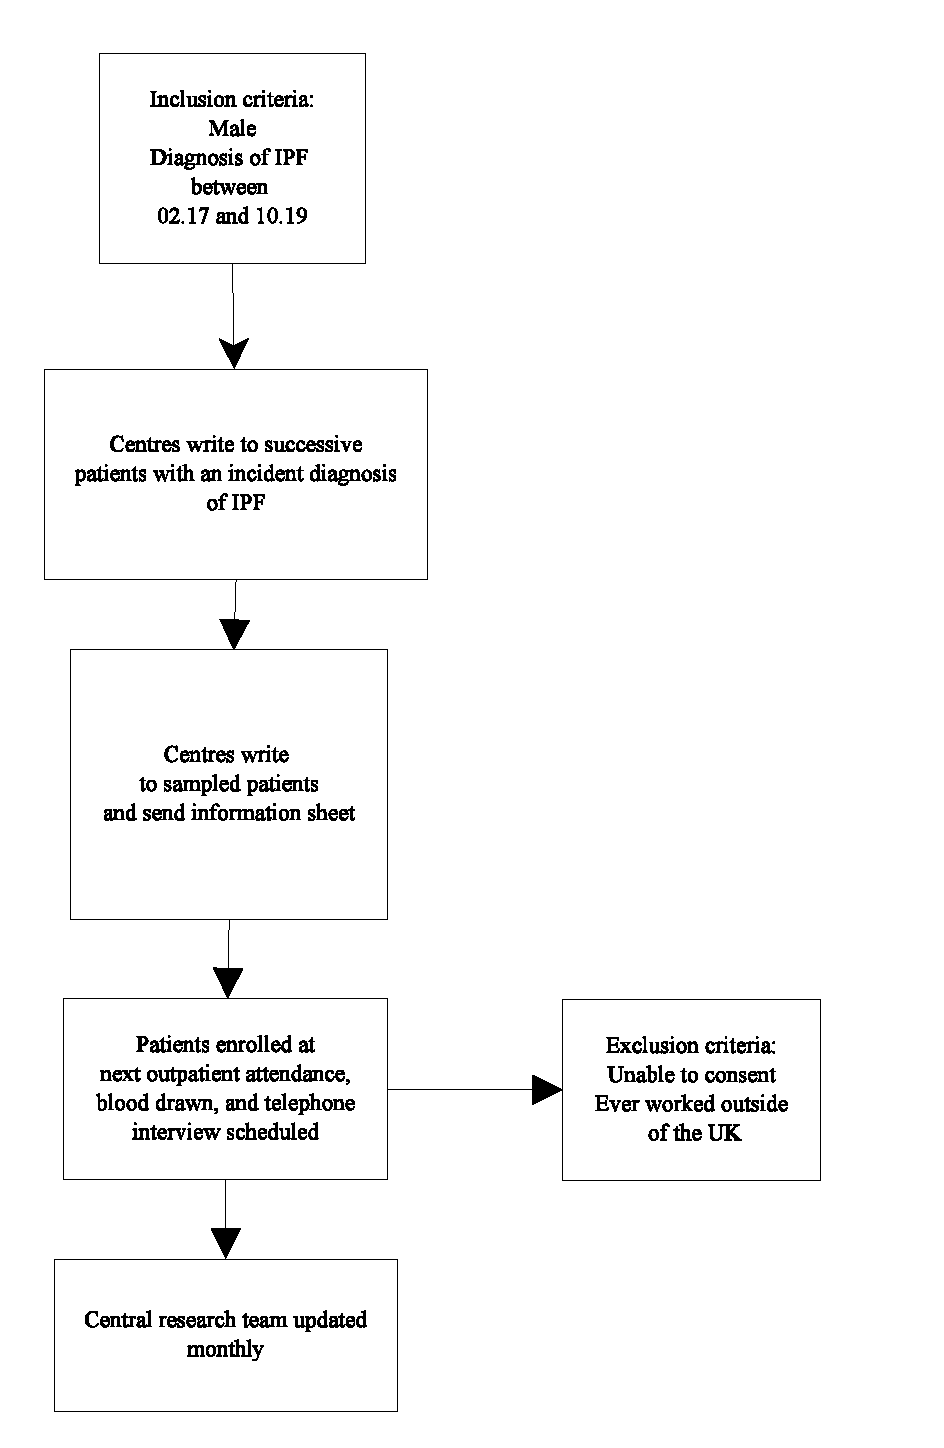
\includegraphics[scale=0.8]{fig/case-recruitment.eps}
\caption{Case recruitment\label{fig:caserec}}
\end{figure}
\subsection{Recruitment of controls}

See figure ~\ref{fig:contrec}

Controls will be recruited from male patients with a new outpatient department attendance at the same hospital cases originate from. Four male controls, frequency matched on age, will be recruited for each case.  

Centres within the research network will provide the research team with a list of the outpatient clinics that take place each month to include details of who the lead clinician is for each clinic, average list size, average new to follow up ratio, and when the clinic runs.

The research team will list each clinic alphabetically and serially assign an integer range equal to the expected number of new patients for each clinic per month. The full integer range will then be randomly shuffled and used to derive a list of clinics from which controls will be recruited sequentially. For example, if a particular TB clinic appeared first on the list then all new male patients attending this clinic within the target age range would be approached to participate as controls. If four controls could not be found from the TB clinic then the same would be repeated at the next clinic on the list.

The research team will write to the lead clinician for selected clinics to obtain permission to recruit patients to the study. Potential controls will be invited to participate in the study and provided with a patient information sheet when they attend the outpatient department. Patients will be enrolled into the study at their next outpatient department attendance, blood will be drawn, and a telephone interview will be scheduled. Inclusion and exclusion criteria will be checked as
part of enrolment.

Recruitment of controls from a centre stops when recruitment of cases stops and four controls for each case have been recruited.

\begin{figure}
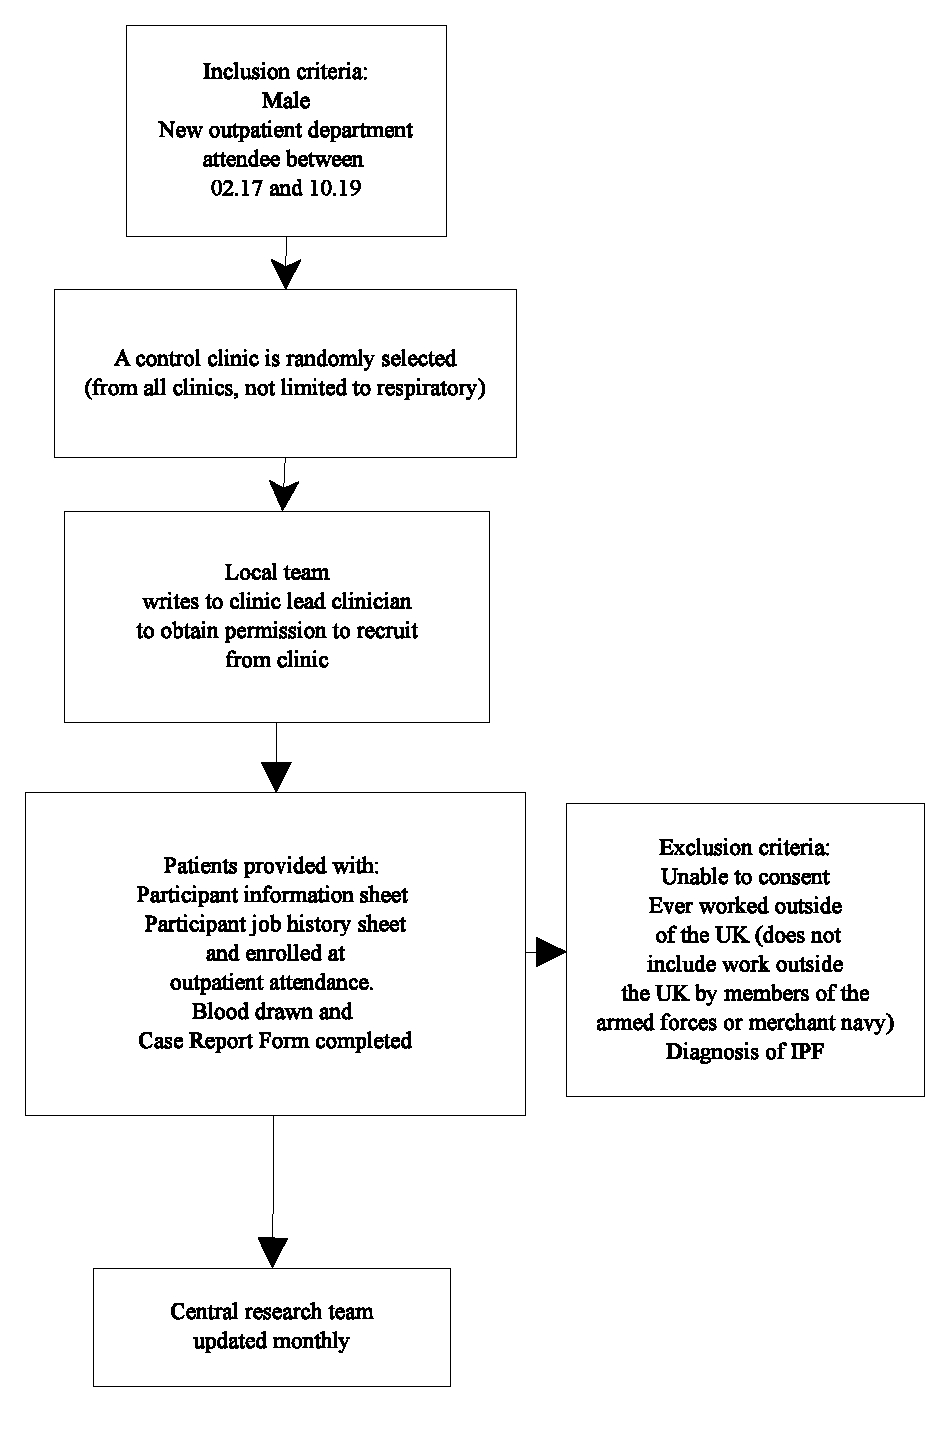
\includegraphics[scale=0.8]{fig/control-recruitment.eps}
\caption{Control recruitment\label{fig:contrec}}
\end{figure}

\section{Exposure assessment}

\subsection{Introduction}

Hello, my name is \textbf{name of researcher}. I am a doctor/nurse/research assistant calling as part of the IPF Job Exposure Study. Is this \textbf{name of participant}? 

I would like to ask you some questions about the jobs you have had, where you have lived, and your lifetime smoking history. I would also like to record this call for our research if that's ok with you.  

Your answers will help us to understand the causes of IPF, make sure people get the right treatment, and ensure that controls of exposures at work are right so that we protect workers and prevent disease in the future.  

The interview should take about 30 minutes. Is now a good time to talk?

\subsection{Occupational and residential history} 

I want you to think about all of the jobs you've had. 

Do you remember the first job that you had after school?

\begin{enumerate}
\item  What was the name of your job?
\item  What did you do in this job?
\item  What did the company make (if applicable)?
\item  Do you remember how old you were or what year you started the job?
\item  Do you remember how old you were or what year you finished the job?
\item  Do you remember where you lived when you had that job?
\item  Do you remember what job you had next?
\end{enumerate}

(1 through 7 repeats until lifetime occupational history is complete. Standard occupational classification is used to code occupations)

`Trigger' jobs prompt more detailed questioning regarding job process(es), materials used, and control measures (according to validated semi-structured job process based historic job exposure assessment tool developed by John Cherrie)

\begin{enumerate}[resume]
\item What country were you born in? 
\item What place were you born in?
\item Do you remember the places you lived when you were growing up? (until you finished school) 
\item When you were growing up who lived at home with you?
\item How long for?
\item Do you remember what their job was?
\end{enumerate}

\subsection{Smoking history}

\begin{enumerate}
\item Have you ever smoked?
\item What old were you when you started smoking?
\item Do you still smoke?
\item How old were you, or when, did you stop smoking?
\item How many, on average, a day do you/did you smoke?
\item What do you/did you smoke?
\end{enumerate}

\subsection{mMRC dyspnoea questions} 

I would like to ask you some questions about being short of breath.

Are you:

\begin{enumerate}
\item Not troubled by breathless except on strenuous exercise?
\item Short of breath when hurrying on a level or when walking up a slight hill?
\end{enumerate}

Are you someone who:

\begin{enumerate}[resume]
\item Walks slower than most people on the level, stops after a mile or so, or stops after 15 minutes walking at own pace?
\item Stops for breath after walking about 100 yds or after a few minutes on level ground?
\end{enumerate}

Are you:

\begin{enumerate}[resume]
\item Too breathless to leave the house, or breathless when dressing/undressing?
\end{enumerate}

\subsection{(for cases only) how were you diagnosed}

\begin{enumerate}
\item What took you to the doctor at the beginning of the illness? 
\end{enumerate}

\section{Venepuncture, sample storage, transportation, and processing} 

Venepuncture will be performed by a qualified practitioner. The number of blood tubes to be drawn depends on the volume of the tubes used. A total of 14mls of blood will be obtained using purple top EDTA containers and a total of 10mls of blood using gold top SST tubes for each participant. Samples will be labelled with the participants unique research ID and posted using Royal Mail Safebox to a secure lab storage facility at NHLI where they will be kept in a -80 degree centigrade freezer.
The sender will record the day of delivery and the research team will record receipt of the sample and keep an accurate record of its location. Analysis of samples will include DNA isolation and quantitative PCR taqman assay to investigate pre-defined SNPs of interest.


\end{document}


